
\begin{frame}[ctb!]
  \frametitle{Cyder Paradigm : Modularity }
  A modular repository framework facilitates 
  \begin{itemize}
    \item  interchangable subcomponents (e.g. buffer material) so that 
      the impact on the disposal system performance may be observed
    \item and simulations with varying levels of detail.
  \end{itemize}
 \pause
  Integration with a fuel cycle simulator facilitates
  \begin{itemize}
    \item analysis of feedback effects upon the fuel cycle
    \item and investigation of fuel cycle choices on disposal system 
      performance.
  \end{itemize}
\end{frame}


\begin{frame}[ctb!]
  \frametitle{Cyder Paradigm : Waste Stream Acceptance}
  \footnotesize{
  
To participate in fuel cycle simulation, the repository model must accept arbitrary 
spent fuel and high level waste streams. A waste stream is a material data 
object resulting from the Cyclus simulated fuel cycle.  
  \begin{figure}[htbp!]
    \begin{center}
      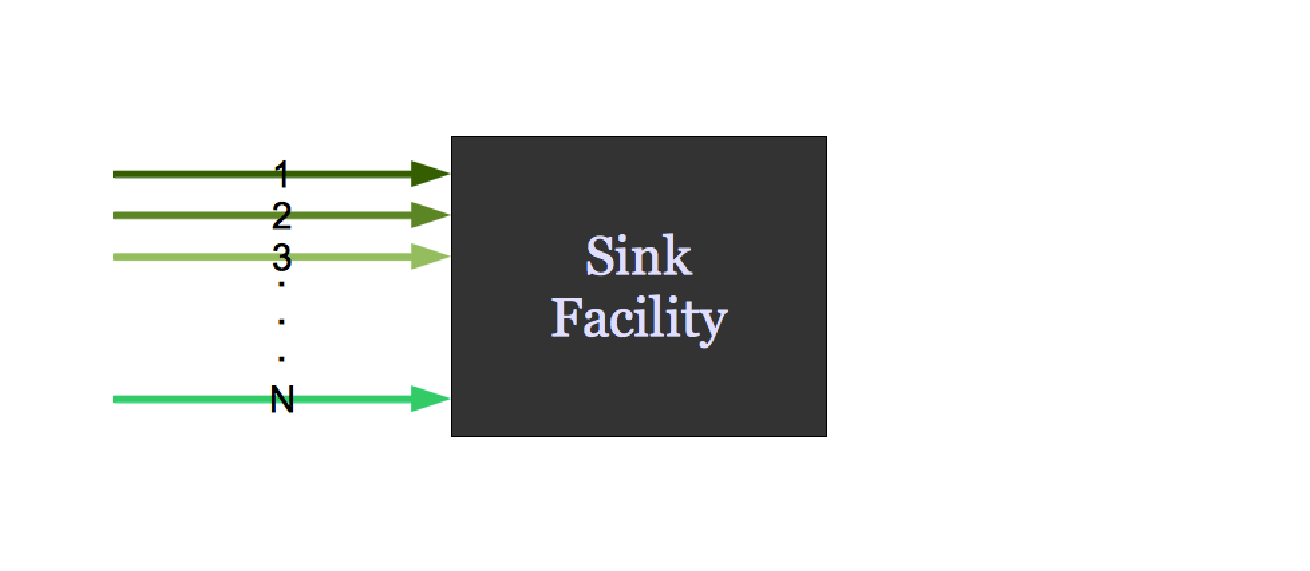
\includegraphics[height=5cm]{./images/sinkfacility.eps}
    \end{center}
    \caption{ The Cyder Facility dynamically accepts material from the 
    coupled fuel cycle simulation.} 
    \label{fig:sinkfacility}
  \end{figure}
% Sink Facility ?
}
\end{frame}

\begin{frame}[ctb!]
  \frametitle{Cyder Paradigm : Waste Stream Conditioning}
  \footnotesize{

    \textbf{Waste conditioning} is the process of packing a waste stream into an appropriate 
waste form.  The Cyder model loads discrete waste forms with discrete waste 
stream contaminant vectors as depicted in Figure \ref{fig:ws_conditioning}.
  
\begin{figure}[htbp!]
\begin{center}
\def\svgwidth{.5\textwidth}
\input{./images/ws_conditioning.eps_tex}
\end{center}
\caption{Waste streams are conditioned into the appropriate waste form 
according to user-specified pairings.}
\label{fig:ws_conditioning}
\end{figure}
}
\end{frame}

\begin{frame}[ctb!]
  \frametitle{Cyder Paradigm : Waste Form Packaging}
  \footnotesize{

    \textbf{Waste packaging} is the process of placing one or many waste forms into a 
containment package. Once the waste stream has been conditioned into a waste 
form, that waste form Component is loaded into a waste package Component as 
depicted in Figure \ref{fig:wf_packaging}.  

\begin{figure}[htbp!]
\begin{center}
\def\svgwidth{.5\textwidth}
\input{./images/wf_packaging.eps_tex}
\end{center}
\caption{Waste forms are loaded into the appropriate waste package 
according to user-specified pairings.}
\label{fig:wf_packaging}
\end{figure}
}
\end{frame}

\begin{frame}[ctb!]
  \frametitle{Cyder Paradigm : Waste Package Emplacement}
\footnotesize{
  \begin{columns}[c]
    \column{0.3\linewidth}
Finally, the waste package is \textbf{emplaced} in a buffer component, which 
contains many other waste packages, spaced evenly in a grid. The grid is 
defined by the user input and depends on repository depth, $\Delta z$, waste 
package spacing, $\Delta x$, and tunnel spacing, $\Delta y$ as in Figure 
\ref{fig:repo_layout}.

    \column{0.6\linewidth}
\begin{figure}[htbp!]
\begin{center}
\def\svgwidth{.5\textwidth}
\input{./images/repo_layout.eps_tex}
\end{center}
\caption{The repository layout has a depth and a uniform package spacing.}
\label{fig:repo_layout}
\end{figure}
\end{columns}
  }
\end{frame}


\begin{frame}
  \frametitle{Nested Components}
  Each Component has : 
  \begin{itemize}
    \item a Geometry to describe its dimensions and location
    \item a NuclideModel for contaminant transport 
    \item a ThermalModel for heat transport
    \item a Parent Component at its external barrier
    \item one or more Daughter Components at its internal barrier
  \end{itemize}

  Components have other data members such as a Type (WF, WP, BUFFER, FF), a 
  material data table, a start date, etc. 
\end{frame}

\begin{frame}
  \frametitle{Nested Components}
  The NuclideModel in a Component can be interchangeably represented by any of 
  the four nuclide transport models. 
    \begin{itemize}
      \item Degradation Rate Based Failure Model
      \item Mixed Cell with Degradation, Sorption, Solubility Limitation
      \item Lumped Parameter Model
      \item 1D Advection Dispersion Solution
    \end{itemize}
\end{frame}

